\documentclass{beamer}
\usetheme[pageofpages=of,% String used between the current page and the
                         % total page count.
          bullet=circle,% Use circles instead of squares for bullets.
          titleline=true,% Show a line below the frame title.
          alternativetitlepage=true,% Use the fancy title page.
	  titlepagelogo=logo-circl.pdf,% Logo for the first page.
%          watermark=watermark-polito,% Watermark used in every page.
%          watermarkheight=100px,% Height of the watermark.
%          watermarkheightmult=4,% The watermark image is 4 times bigger
                                % than watermarkheight.
          ]{Torino}

\usepackage[utf8x]{inputenc}
\usepackage{listings}
\usepackage{soul}
\usepackage{siunitx}
\usepackage{booktabs}
%\lstset{ 
%  backgroundcolor=\color{white},   % choose the background color; you must add \usepackage{color} or \usepackage{xcolor}
%  basicstyle=\footnotesize,        % the size of the fonts that are used for the code
%  breakatwhitespace=false
%}

\usepackage{tikz}
\usetikzlibrary{shapes,snakes,automata,positioning,matrix,fit,arrows,shapes.geometric}


\usepackage[listings]{tcolorbox}
\usepackage{xcolor}
\usepackage{colortbl}
\definecolor{mygreen}{rgb}{0,0.6,0}
\definecolor{mygreen2}{rgb}{0,0.56,0.16}
\definecolor{myred}{rgb}{0.6,0.066,0.066}
\definecolor{redCIRCL}{RGB}{213,43,30}
\definecolor{mygray}{rgb}{0.5,0.5,0.5}
\definecolor{mymauve}{rgb}{0.58,0,0.82}
\definecolor{mygray}{gray}{0.9}
\definecolor{mywhite}{rgb}{1,1,1}
\definecolor{myblack}{rgb}{0,0,0}
\definecolor{mybeige}{HTML}{eeeeee}
%\usepackage{tcolorbox}
\usepackage[listings]{tcolorbox}
\tcbuselibrary{listings}

\lstdefinestyle{code}{ %
  backgroundcolor=\color{mybeige},   % choose the background color; you must add \usepackage{color} or \usepackage{xcolor}; should come as last argument
  basicstyle=\footnotesize\ttfamily,        % the size of the fonts that are used for the code
  breakatwhitespace=false,         % sets if automatic breaks should only happen at whitespace
  breaklines=true,                 % sets automatic line breaking
  captionpos=b,                    % sets the caption-position to bottom
  commentstyle=\color{mygreen},    % comment style
  deletekeywords={...},            % if you want to delete keywords from the given language
  escapeinside={\%*}{*)},          % if you want to add LaTeX within your code
  extendedchars=true,              % lets you use non-ASCII characters; for 8-bits encodings only, does not work with UTF-8
  frame=single,	                   % adds a frame around the code
  keepspaces=true,                 % keeps spaces in text, useful for keeping indentation of code (possibly needs columns=flexible)
  keywordstyle=\color{blue},       % keyword style
  language=Python,                 % the language of the code
  morekeywords={*,...},           % if you want to add more keywords to the set
  numbers=left,                    % where to put the line-numbers; possible values are (none, left, right)
  numbersep=5pt,                   % how far the line-numbers are from the code
  numberstyle=\tiny\color{myblack}, % the style that is used for the line-numbers
  rulecolor=\color{black},         % if not set, the frame-color may be changed on line-breaks within not-black text (e.g. comments (green here))
  showspaces=false,                % show spaces everywhere adding particular underscores; it overrides 'showstringspaces'
  showstringspaces=false,          % underline spaces within strings only
  showtabs=false,                  % show tabs within strings adding particular underscores
  stepnumber=1,                    % the step between two line-numbers. If it's 1, each line will be numbered
  stringstyle=\color{mymauve},     % string literal style
  tabsize=2,	                   % sets default tabsize to 2 spaces
  title=\lstname                   % show the filename of files included with \lstinputlisting; also try caption instead of title
}
\lstdefinestyle{bash}{ %
  backgroundcolor=\color{black!85},   % choose the background color; you must add \usepackage{color} or \usepackage{xcolor}; should come as last argument
  basicstyle=\footnotesize\color{mywhite},        % the size of the fonts that are used for the code
  breakatwhitespace=false,         % sets if automatic breaks should only happen at whitespace
  breaklines=true,                 % sets automatic line breaking
  captionpos=b,                    % sets the caption-position to bottom
  commentstyle=\color{mygreen},    % comment style
  deletekeywords={...},            % if you want to delete keywords from the given language
  escapeinside={\%*}{*)},          % if you want to add LaTeX within your code
  extendedchars=true,              % lets you use non-ASCII characters; for 8-bits encodings only, does not work with UTF-8
  frame=single	                   % adds a frame around the code
  keepspaces=true,                 % keeps spaces in text, useful for keeping indentation of code (possibly needs columns=flexible)
  keywordstyle=\color{white}\bfseries,       % keyword style
  language=bash,                 % the language of the code
  morekeywords={*,$,git, clone,... },           % if you want to add more keywords to the set
  numbers=left,                    % where to put the line-numbers; possible values are (none, left, right)
  numbersep=5pt,                   % how far the line-numbers are from the code
  numberstyle=\tiny\color{mywhite}, % the style that is used for the line-numbers
  rulecolor=\color{black},         % if not set, the frame-color may be changed on line-breaks within not-black text (e.g. comments (green here))
  showspaces=false,                % show spaces everywhere adding particular underscores; it overrides 'showstringspaces'
  showstringspaces=false,          % underline spaces within strings only
  showtabs=false,                  % show tabs within strings adding particular underscores
  stepnumber=1,                    % the step between two line-numbers. If it's 1, each line will be numbered
  stringstyle=\color{mymauve},     % string literal style
  tabsize=2,	                   % sets default tabsize to 2 spaces
  title=\lstname                   % show the filename of files included with \lstinputlisting; also try caption instead of title
}
\lstdefinestyle{default}{ %
  backgroundcolor=\color{white},   % choose the background color; you must add \usepackage{color} or \usepackage{xcolor}; should come as last argument
  basicstyle=\footnotesize\color{black},        % the size of the fonts that are used for the code
  breakatwhitespace=false,         % sets if automatic breaks should only happen at whitespace
  breaklines=true,                 % sets automatic line breaking
  captionpos=b,                    % sets the caption-position to bottom
  commentstyle=\color{mygreen},    % comment style
  deletekeywords={...},            % if you want to delete keywords from the given language
  escapeinside={\%*}{*)},          % if you want to add LaTeX within your code
  extendedchars=true,              % lets you use non-ASCII characters; for 8-bits encodings only, does not work with UTF-8
  frame=single	                   % adds a frame around the code
  keepspaces=true,                 % keeps spaces in text, useful for keeping indentation of code (possibly needs columns=flexible)
  keywordstyle=\color{white}\bfseries,       % keyword style
  language=bash,                 % the language of the code
  morekeywords={*,$,git, clone,... },           % if you want to add more keywords to the set
  numbers=left,                    % where to put the line-numbers; possible values are (none, left, right)
  numbersep=5pt,                   % how far the line-numbers are from the code
  numberstyle=\tiny\color{black}, % the style that is used for the line-numbers
  rulecolor=\color{black},         % if not set, the frame-color may be changed on line-breaks within not-black text (e.g. comments (green here))
  showspaces=false,                % show spaces everywhere adding particular underscores; it overrides 'showstringspaces'
  showstringspaces=false,          % underline spaces within strings only
  showtabs=false,                  % show tabs within strings adding particular underscores
  stepnumber=1,                    % the step between two line-numbers. If it's 1, each line will be numbered
  stringstyle=\color{mymauve},     % string literal style
  tabsize=2,	                   % sets default tabsize to 2 spaces
  title=\lstname                   % show the filename of files included with \lstinputlisting; also try caption instead of title
}
\lstset{style=code}


\AtBeginSection[]{
  \begin{frame}
  \vfill
  \centering
  \begin{beamercolorbox}[sep=8pt,center,shadow=true,rounded=true]{title}
      {\color{white} \usebeamerfont{title}\insertsectionhead}\par%
  \end{beamercolorbox}
  \vfill
  \end{frame}
}

\author{\Large{Alexandre Dulaunoy}\\ \scriptsize{alexandre.dulaunoy@circl.lu}\\ \large{Aurelien Thirion}\\ \scriptsize{aurelien.thirion@circl.lu}\\ \large{Jean-Louis Huynen}\\ \scriptsize{jean-louis.huynen@circl.lu}\\}
\title{Darknet and Social Network Monitoring}
\subtitle{Introduction to Challenges, Concepts and Data Mining of the Deep Web}
\institute{info@circl.lu}
\date{\today}

\begin{document}


\begin{frame}[t,plain]
\titlepage
\end{frame}

\begin{frame}
 % \frametitle{CIRCL}
 
\includegraphics[scale=0.5]{logo-circl.pdf}
 \begin{itemize}
 \item The Computer Incident Response Center Luxembourg (CIRCL) is a government-driven initiative designed to provide a systematic response facility to computer security threats and incidents.
 \item CIRCL is the CERT for the private sector, communes and non-governmental entities in Luxembourg.
 \end{itemize}
\end{frame}

\begin{frame}{CIRCL Missions 1/2}
\begin{itemize}
\item Provide a {\bf systematic response} facility to ICT-incidents;
\item Support national ICT users to {\bf recover quickly and efficiently} from security incidents;
\item {\bf Minimize ICT incident-based losses}, theft of information and disruption of services for the private sector;
\end{itemize}
\end{frame}

\begin{frame}{CIRCL Missions 2/2}
\begin{itemize}
\item Gather information related to incident handling to better {\bf prepare future incidents} management and provide optimized protection for systems and data;
\item {\bf Coordinate communication} among national and international incident response teams during security emergencies and to help prevent future incidents;
\item Provide a security related {\bf alert and warning system} for organisations in Luxembourg and abroad;
\item Foster {\bf knowledge and information} exchange in cybersecurity {\bf lead the development of MISP project};
\end{itemize}
\end{frame}


\begin{frame}
\frametitle{Links}
    \begin{itemize}
        \item AIL project: \url{https://github.com/ail-project}
        \item AIL framework: \url{https://github.com/ail-project/ail-framework}
        \item Training materials: \url{https://github.com/ail-project/ail-training}
        \item Online chat: \url{https://gitter.im/ail-project/community}
    \end{itemize}
\end{frame}


\begin{frame}
        \frametitle{Ethics in Information Security and Cybersecurity}
        \begin{itemize}
        \item The materials and tools presented can open a significant numbers of questions regarding ethics;
        \item Our researches and tools are there for education, supporting the public good and improve incident response;
        \item We ask all users and participants to {\bf follow ethical principles and act professionaly}\footnote{\url{https://www.acm.org/code-of-ethics} \url{https://www.first.org/global/sigs/ethics/ethics-first}}.
        \end{itemize}
\end{frame}

\begin{frame}
        \frametitle{Privacy, AIL and GDPR (PII) - An Ethical Question}
        \begin{itemize}
                \item Many modules in AIL can process personal data and even special categories of data as defined in GDPR (Art. 9).
                \item The data controller is often the operator of the AIL framework (limited to the organisation) and has to define {\bf legal grounds for processing personal data}.
                \item To help users of AIL framework, a document is available which describe points of AIL in regards to the regulation\footnote{\url{https://www.circl.lu/assets/files/information-leaks-analysis-and-gdpr.pdf}}.
        \end{itemize}
\end{frame}

\section{Objectives}
\begin{frame}
\frametitle{Our objectives}
    \begin{itemize}
        \item Provide a quick overview to darknet, deep web, collection and cyber threat intelligence lifecycle;
        \item Review different {\bf collection mechanisms} and {\bf sources};
        \item Some practical examples of criminal activities and their use of modern technologies;
        \item Show the benefits of developing open source tools to monitor web pages, pastes, forums and hidden services;
        \item Quick introduction to the open source AIL project;
    \end{itemize}
\end{frame}

\section{Introduction}
\begin{frame}
        \frametitle{Concepts - Deep Web}
        \begin{itemize}
                \item {\bf Deep Web} is the part of World Wide Web not indexed or directly accessible by standard web search-engines;
                \item This can be content hidden from {\bf crawlers} by requiring a specific access and this can includes private social media, password-protected forums or content protected
                        by different measures such as paywalls or specific security interface to access the information;
                \item A large portion of content accessible via Internet is part of the deep web\footnote{also called invisible web, hidden web or non-indexed web}.
        \end{itemize}
\end{frame}

\begin{frame}
        \frametitle{Concepts - darknet}
        \begin{itemize}
                \item {\bf Darknet} is an overlay network running on top of Internet requiring specific software to access the network and its services;
                \item Tor, I2P and Freenet are the most commonly used ones. Many are used for hidden services access and some for proxy access to the Internet;
		\item There are {\bf legitimate use-cases} for such network but also many {\bf illegal or criminal usage}.
        \end{itemize}
\end{frame}

\begin{frame}
	\frametitle{Collection and Sources}
	\begin{itemize}
		\item Collection (mainly OSINT\footnote{public or open source sources} or covert/clandestine sources) is the act of gathering manually or automatically data from different sources;
		\item {\bf Determining and maintaining the sources}:
		\begin{itemize}
			\item Hidden services (on Tor) such as forums, market places, chatrooms, public site\footnote{\url{https://github.com/ail-project/ail-splash-manager}}...
			\item Social network (e.g. Twitter) from Twitter\footnote{\url{https://github.com/ail-project/ail-feeder-twitter}} to Instagram.
			\item Chat and discussion forum from Discord, Telegram\footnote{\url{https://github.com/ail-project/ail-feeder-telegram}} and private hidden one on Tor or other overlay networks.
			\item News and security reports\footnote{\url{https://github.com/ail-project/ail-feeder-atom-rss}}.
		\end{itemize}
	\end{itemize}
\end{frame}

\begin{frame}
	\frametitle{Lifecycle of collection and analysis}
	\center
\tikzstyle{startstop} = [rectangle, rounded corners, minimum width=3cm, minimum height=0.8cm,text centered, draw=black, fill=red!30]
\tikzstyle{io} = [trapezium, trapezium left angle=70, trapezium right angle=110, minimum width=3cm, minimum height=1cm, text centered, draw=black, fill=blue!30]
\tikzstyle{arrow} = [thick,->,>=stealth]
	\begin{tikzpicture}[node distance=1.4cm]

\node (start) [startstop] {Planning};
\node (collect) [startstop, below of =start] {Collect};
\node (processing) [startstop, below of =collect] {Processing};
\node (analysing) [startstop, below of=processing] {Analysing};
\node (dissemination) [startstop, below of=analysing] {Dissemination};
\draw [arrow] (start) -- (collect);
\draw [arrow] (collect) -- (processing);
\draw [arrow] (processing) -- (analysing);
\draw [arrow] (analysing) -- (dissemination);
%\draw [arrow] (analysing) |- (collect);
\end{tikzpicture}

\end{frame}

\begin{frame}
        \frametitle{Collecting, processing and analysing content - web pages}
        \begin{itemize}
		\item Building a search engine on the web is a challenging task because:
        	\begin{itemize}
			\item it has to crawl webpages,
			\item it has to to make sense of {\bf unstructured data},
			\item it has to {\bf index} these data,
			\item it has to provide a way to retrieve data and structure data (e.g. correlation).
        	\end{itemize}
		\item Doing so on Tor is even more challenging because:

        	\begin{itemize}
			\item services don't always want to be found,
			\item parts of the dataset have to be discarded.
        	\end{itemize}
	\item in each case, it requires a lot of bandwidth, storage and computing power.
        \end{itemize}
\end{frame}

\section{Demo of analysed content}

\section{Tor - a detailed overview of an overlay network}
\begin{frame}
        \frametitle{Concepts - tor}
        \begin{itemize}
		\item tor makes use of {\bf onion routing} to obfuscate user identify,
        \end{itemize}
	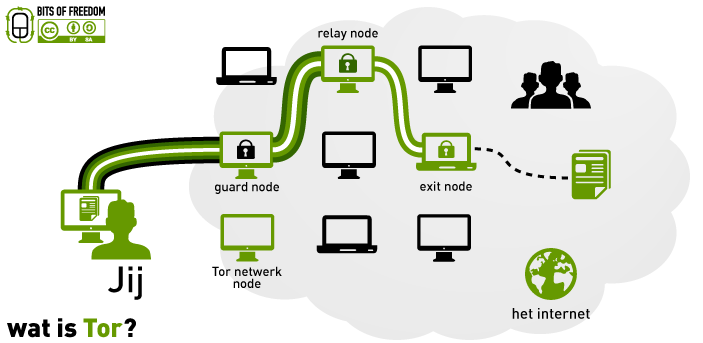
\includegraphics[scale=0.5]{images/tor1.png}
\end{frame}


\begin{frame}
        \frametitle{Concepts - tor}
	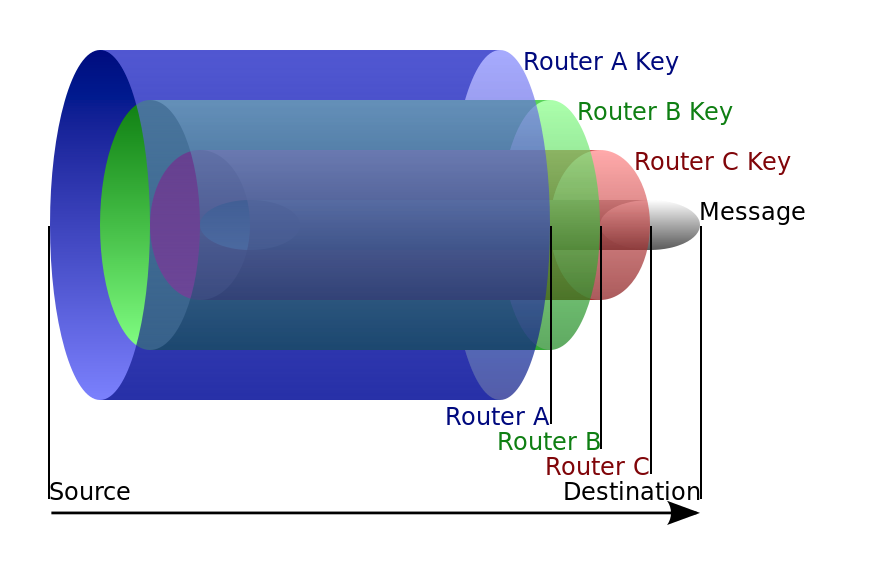
\includegraphics[scale=0.3]{images/tor2.png}
\end{frame}

\begin{frame}
        \frametitle{Concepts - tor}
	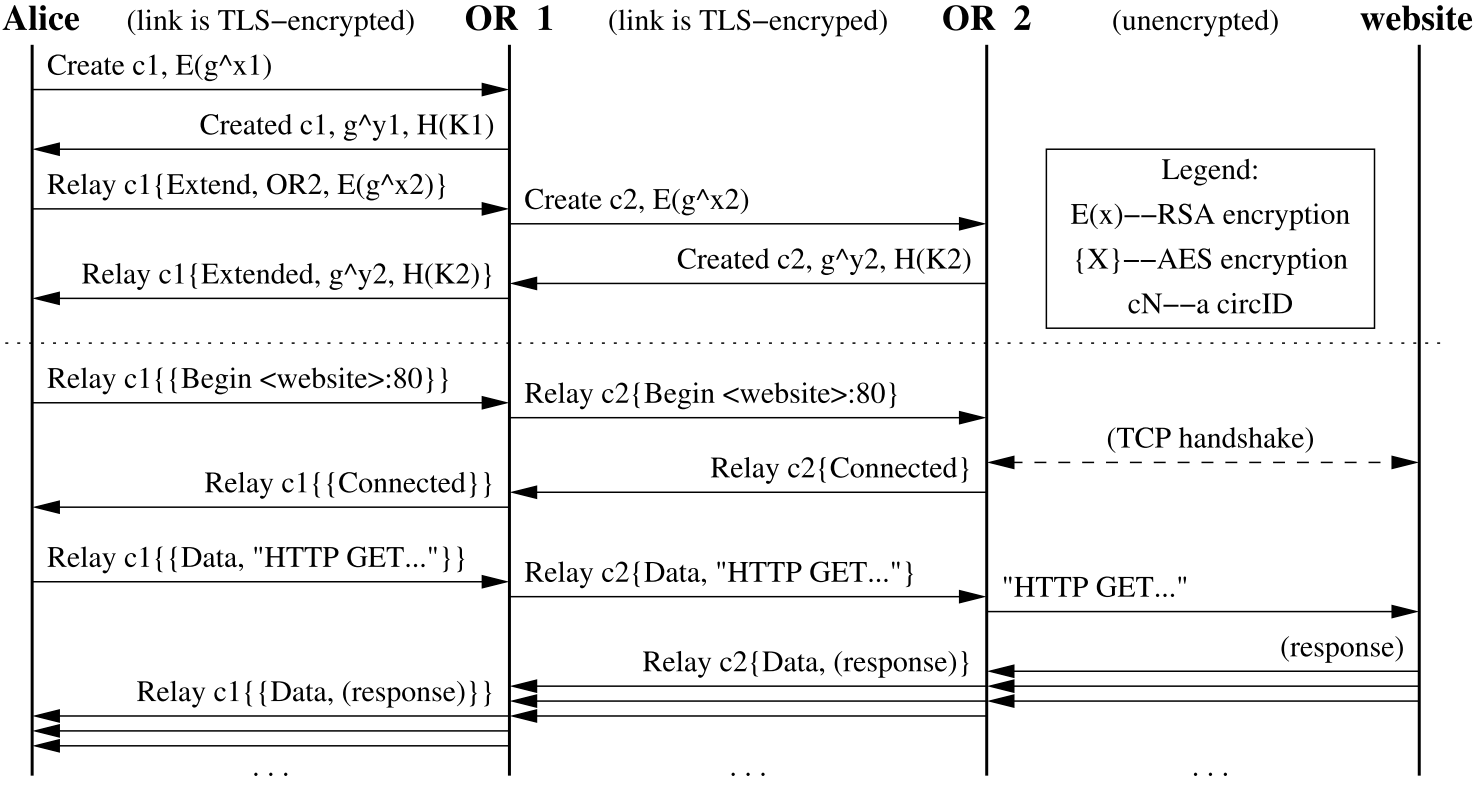
\includegraphics[scale=0.3]{images/tor3.png}
\end{frame}


\begin{frame}
        \frametitle{Concepts - tor}
        \begin{itemize}
		\item tor provide hidden services: addresses in {\bf.onion},
		\item one can only reach such service when one knows its address,
		\item hidden services' information are stored in a {\bf Distributed Hash Table},
		\item these are really interesting for attackers as:
        	\begin{itemize}
		\item these are anonymous,
		\item these can be provided through NATs,
		\item these can be moved easily.
        	\end{itemize}
        \end{itemize}
\end{frame}

\end{document}

